\documentclass[b5paper,11pt]{article}
\bibliographystyle{plain}

\usepackage{geometry}
\usepackage{amssymb,amsthm,bm,mathrsfs,mathtools}
\usepackage[usenames]{xcolor}
\usepackage{hyperref}
\usepackage{graphicx}
\graphicspath{{../"img/"}{../"figures/"}}

\usepackage{mycommands}
\newcommand{\numcircled}[1]{\raisebox{.5pt}{\textcircled{\raisebox{-.9pt} {#1}}}}
\newcommand{\Dmax}{\trdis_\mathsf{max}}
\newcommand{\InFmax}{\infid_\mathsf{max}}
\newcommand{\Psb}{\mathcal{P}_\mathrm{SB}}
\newcommand{\Odd}{\Omega_{\mathsf{DD}}}
% \newcommand{F}{\Omega_{\mathsf{PDD}}}
\newcommand{\vOpdd}{\vec{\Omega}_{\mathsf{P}}}
\newcommand{\LO}[1]{\operatorname{LO}}
\newcommand{\alphat}{\widetilde{\alpha}}
\newcommand{\betat}{\widetilde{\beta}}
\newcommand{\wt}[1]{\widetilde{#1}}
\newcommand{\Ppb}{\mathscr{P}_{\mathrm{0}}}
\newcommand{\Pcp}{\mathscr{P}_{\mathrm{c}}}
\newcommand{\wtP}{\widetilde{P}}
\newcommand{\wtH}{\widetilde{H}}
\newcommand{\wtO}{\widetilde{\Omega}}
\newcommand{\wtU}{\widetilde{U}}

\newcommand{\HB}{H_\mathrm{B}}
\newcommand{\HSB}{H_\mathrm{SB}}

\newcommand{\Heff}{H_\mathrm{eff}}
\newcommand{\HeffB}{H_\mathrm{eff,B}}
\newcommand{\HeffSB}{H_\mathrm{eff,SB}}

\newcommand{\ep}{\Phi_\mathrm{SB}}
\newcommand{\wtep}{\widetilde{\Phi}_\mathrm{SB}}
\newcommand{\epB}{\Phi_\mathrm{B}}
\newcommand{\phiB}{\phi_\mathrm{B}}

\newcommand{\CDDn}{\textsf{CDD\textsubscript{n}}}
\newcommand{\rDD}{\mathrm{DD}}
\newcommand{\rmax}{\mathrm{max}}
\begin{document}
\section{Scaling up protection}\label{sec:threshold}
\blue{(Generalization of the previous PDD section; CDD content from Secs.~IVA-D of draft by Jiaan \& Xiansong. The main goal here is to show that an accuracy threshold for DD, under the CDD scheme for scaling up, fails to exist. This means that there is a maximum level for CDD, beyond which further levels only make things worse. To discuss the differences from using different measures.)}
We can distinguish between two operational considerations: to preserve states in a quantum memory (no computational gates), or to reduce noise in the course of carrying out a quantum computation. In the memory setting, the goal is to preserve the quantum informational state for some time $T$ without damage. During this time $T$, we can do DD pulses, and ask if the noise at the end of each complete DD sequence is lower than the noise over the same time period if there were no DD pulses. In other words, for DD to work well, we require
\begin{equation}
\textrm{Memory setting:}\quad \epsilon_\mathrm{DD}<\epsilon(L),
\end{equation}
where $\epsilon_\mathrm{DD}$ quantifies the noise after the DD sequence, while $\epsilon(L)$ is the noise after bare evolution for the time taken for the $L$ DD pulses to be applied.
In the computational setting, the comparison of with and without DD is different. With DD, computational gates can only be applied at the completion of each iteration of the DD sequence, as opposed to every time step without DD. The condition for DD to be effective in this case is then
\begin{equation}\label{eq:cond}
\textrm{Computational setting:}\quad\epsilon_\mathrm{DD}<\epsilon(1),
\end{equation}
where $\epsilon(1)$ is the noise after bare evolution for a single time step. 

\begin{figure}[htbp]
 \centering
 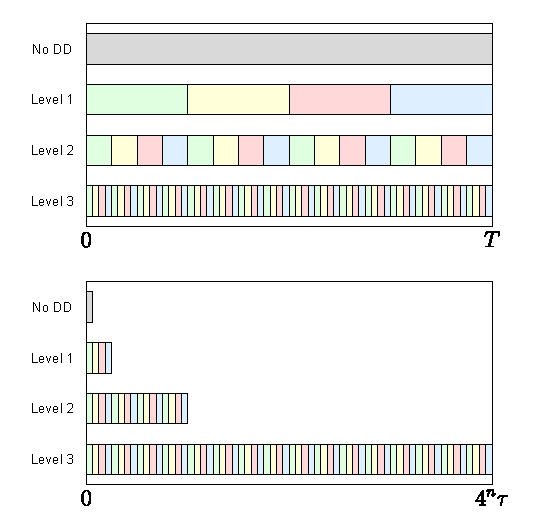
\includegraphics[width=\linewidth]{memory-vs-computation}
 \caption{\blue{An illustration of the CDD time evolution maps under increasing concatenation levels.  We compare the quantum memory setting (above) to the quantum computation setting (under).}}
 \label{fig:memvscom}
\end{figure}

\blue{These two perspectives result in very different overall decoupling strategies. Especially if one is using CDD to ``scale up protection''. As illustrated in Fig.~\ref{fig:memvscom}, for the quantum memory setting, as total time is fixed $T$, one only need to come up with finer and finer slicing of the time evolution pieces; but for the quantum computation setting, one need to join the DD control gates to form a dilated time evolution map. The past papers in favor of CDD had taken the former perspective. It is undeniable that with finer and finer slicing of time evolution, one gets better and better performance. But this picture has some series drawbacks. First the total evolution time $T$ is typically unknown, even for quantum memory. Hence there is no way of knowing in advance which gate to perform at what time. Second, there exists a minimal switch/cool-down time between consecutive gates due to 
technological limitations. Hence it is impractical to arbitrarily suppress noise by increasing concatenation level. 
} 

In our work, we focus on the computational setting, the more stringent one among the two, though it is straightforward to modify our analysis for the memory case. As we will see, Condition \eqref{eq:cond} will yield a requirement on the noise parameters characterizing the noise in the system and the DD pulses. We refer to that requirement as the ``break-even point" for DD, borrowing terminology from quantum error correction and fault-tolerant quantum computing.\red{ (There was a comment in the .tex file that some past papers have analyzed the memory case. What are those papers? Do you just mean the Khodjasteh-Lidar 2007 paper? That paper looks only at imperfections due to finite-width pulses, not control errors as we do here. Their paper hence only has a single-parameter $\ep$, not our two-parameter $\ep$ and $\eta$ situation. In fact, in current experiments $\eta$ is likely the larger problem; memory noise is usually much smaller than gate noise. Or are there other earlier papers?)} \blue{(Yes, that paper in particular. Their conclusion that CDD decouples to order $n$ and dramatically outperforms PDD come from this perspective. Our paper is focused on the quantum computation case which is more practical. See my new added picture \ref{fig:memvscom}). And let me quote their words (bottom left page 10) on how they do the comparison: ``The higher order data for PDD are obtained by simply repeating the basic sequence and shrinking the pulse interval. This is necessary to get the long-term behavior of decoupling. \ldots''  I move this memory/computation argument from the previous  section as it is more appropriate when we discuss the scaling behavior.  ---Jiaan)}

\blue{(To be merged with the new text.) }\gray{The conditions for achieving noise suppression are already derived previously for the idealistic PDD and CDD case.
In general, we find that smaller $(\alpha,\beta)$ values would lead to to better noise suppression rate. Therefore the gates should be performed as frequently as possible. But this may leads to suboptimal outcomes in practice given the extra noise introduced by imperfect gate operations. To study the fault-tolerance of DD, we must account for the additional noise associated with the control gates.}



% \subsection{Accuracy Threshold}
We can certainly discuss the break-even point for a particular $\CDDn$ sequence, treating it simply as a ``flattened" sequence of pulses, and ask when the error phase after $\CDDn$ is reduced:
\begin{equation}
 \Phi_{\mathrm{SB},n} < \phi_{\mathrm{SB}},
\end{equation}
 as was done for PDD in the previous section. 
However, what is more interesting is the question of the so-called accuracy threshold for CDD.
As described in the Preliminaries section, CDD achieves higher and higher decoupling order by concatenating the same basic DD scheme---PDD for our discussion here---to higher and higher levels. 
We are interested in understanding how the noise removal improves as the DD scheme scales up.  An accuracy threshold for CDD exists if the parameters governing the noise of the situation satisfying a condition $\eta<\eta_0$, such that 
\begin{equation}\label{eq:thresCond}
\Phi_{\mathrm{SB},n+1} < \Phi_{\mathrm{SB},n}\qquad\forall n=1,2,\ldots.
\end{equation}
In fault-tolerant quantum computing, there is the concept of a fault tolerance noise threshold, a strength of the noise below which scaling up the QEC code leads to improved protection against noise, and hence more accurate quantum computation. This threshold is referred to as the accuracy threshold. Here, we ask the analogous question of CDD, whether there is a condition on the noise parameter of the problem such that increasing the concatenation level always leads to improved noise removal capabilities. 
\blue{If such condition can not be satisfied, we ask the question of whether there exists an optimal concatenation level and how the imperfection in gate control could impact it.}
%

\subsection{Ideal case}
Should the accuracy threshold exist, then \Eqref{eq:thresCond} must first and foremost apply in the case where the gate noise is non-existent. 
 Below, we examine this condition for the ideal CDD before examining on the noisy version.

Following the approach of Khodjasteh and Lidar, the $\CDDn$ generator in the ideal case can be estimated as:
\begin{align}\label{eq:cdd-generator-est}
\Omega_{n} 
\approx {} & \sigma_0 \otimes 4^n B_0 \notag \\
+\ & \sigma_1 \otimes (-\upi)^{n} 2^{n(n+1)} \ad_{B_0}^{n}(B_1)\\ 
+\ & \sigma_2 \otimes (-\upi)^{n} 2^{n^2} \ad_{B_0}^{n-\!1}( \,[B_0,B_2] - \upi \{B_1,B_3\} \,). \notag
\end{align} 
It is shown in the appendix \ref{app:CDD}   that the above expression indeed captures the leading order behavior of $\Omega_{n}$. Hence $\CDDn$ indeed achieves $n$th-order decoupling. Different from the leading order term in the Magnus series, \Eqref{eq:cdd-generator-est} combines the leading order pure bath part and the interaction part. 
The pure bath part, whose size can be estimated by $\Phi_{\mathrm{B},n} \simeq 4^n\phi_\rB$, is of first order; whereas the interaction part is of $(n+1)$th order. 
Focusing on the leading order interaction part, we can derive an upper bound for for the error phase: 
\begin{equation}\label{eq:CDDerrph-ub}
\Phi_{\mathrm{SB},n} \lesssim \,
2^{n(n+2)} \phi_\rB^{n}\,\phi_\rSB \,f_n\!\Bigl(\frac{\phi_\rSB}{\phi_\rB}\Bigr),
\end{equation}
where the auxillary $f_n$ function is defined by:
\begin{equation}
 f_n(x) \equiv\left\{
 \begin{aligned}
 &1, && x \le  \sqrt{4^n-1}, \\
 &\frac{1}{2^n} \sqrt{\left(\frac{4^n-1}{2x}+\frac{x}{2}\right)^2+1}, &&
 x > \sqrt{4^n-1}.
 \end{aligned}
 \right.
\end{equation}
As mentioned in the Preliminaries section, $\CDDn$ achieves $n$th-order decoupling. This can be understood from the error phase expression: $\Phi_{\mathrm{SB},n}$ after $\CDDn$ is of order $\phi^{n+1}$, for $\phi\sim\phi_\rB, \phi_\rSB$. That $\phi_\rB$ enters the error phase should again be of no surprise---as in the PDD case, $\phi_\rB$ determines how quickly the noise seen by the system evolves, and hence affects the efficacy of DD which does a good elimination of the noise only when the noise remains nearly unchanged for the full DD sequence. 

What is perhaps more surprising is the appearance of the $2^{n(n+2)}$ factor in $\Phi_{\mathrm{SB},n}$, a important feature in the CDD. For fixed $\tau_0\equiv \tau$ as $n$ increases (e.g., if $\tau$ is the experimental limit for the switch time between consecutive pulses), such factors mean that the error phase eventually increases for large enough $n$: The exponentially decreasing $\phi^n$ factor is eventually overcome by the super-exponentially increasing $2^{n^2}$ factor. This means there is no accuracy threshold, i.e., there is no level of noise that is weak enough such that $\Phi_{\mathrm{SB},n+1}\leq\Phi_{\mathrm{SB},n}$ for all $n$. Instead, there is an maximal useful level of concatenation level, beyond which further concatenation actually increases the noise seen by the system. Fig.~\ref{fig:estimator-size} plots this situation of fixed $\tau_0$, for increasing concatenation level $n$. We observe the initial decrease of $\Phi_{\mathrm{SB},n}$ as $n$ increases, but this turns around eventually. 

\begin{figure}
    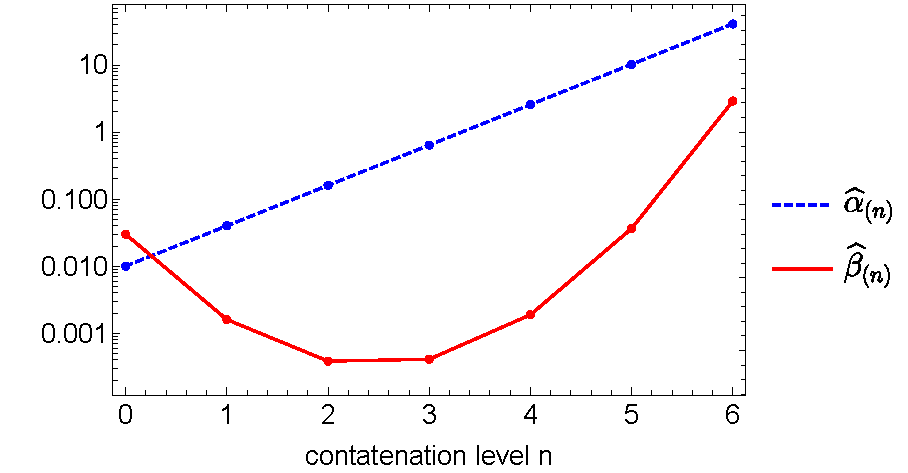
\includegraphics[width=\linewidth]{cdd-estimator}
    \caption{The error phase as a function of the concatenation level. 
    The thin colored lines are obtained from random samples satisfying $\phi_\rB=\phi_\rSB=0.001$. The blue dashed line is our theoretical upper bound for error phase. The maximal concatenation level occurs at 4 in this configuration.}
    \label{fig:estimator-size}
\end{figure}

The upper bound (\ref{eq:CDDerrph-ub}) alone is insufficient 
for predicting when will $\Phi_{\mathrm{SB},n+1} < \Phi_{\mathrm{SB},n} $. As that would require both an upper and lower bound. 
For higher concatenation level to make sense, increasing concatenation level should decrease the error phase. To derive a sufficient condition of it, we examine the recursive relation between concatenation 
levels, which suggests 
\begin{equation}
\begin{aligned}
 B_{n+1,0} &= 4  B_{n,0}\\
 B_{n+1,1} & = -4\upi [B_{n,0}, B_{n,1} ]\\
 B_{n+1,2} & = -2\upi [B_{n,0}, B_{n,1} ]\\
  B_{n+1,3} &=0
\end{aligned}
\end{equation}
For both $B_1$ and $B_2$ to decrease in size, it suffice to require the map 
$-4\upi [B_{n,0},\cdot]$ a contraction map. 
By requiring its norm to be smaller than 1, we obtain the bound for the maximal concatenation level:
\begin{equation}\label{eq:cdd-max-level}
n_{\max}\le -\log_4(\phi_\rB)-3/2.
\end{equation}

Note that the existence of a maximal useful concatenation level does not technically contradict the statement that 
higher-order decoupling is achieved by higher level CDD. Using decoupling order to quantify the degree of noise removal requires, in the first place, the convergence of the Magnus series, so that the $(n+1)$th- and higher-order terms in the series are a small correction to the first $n$ terms. However, if the DD scheme is designed such that the total time for the sequence grows exponentially with $n$, as is the case for CDD if $\tau_0$ is fixed as $n$ increases, eventually, we exceed the convergence criterion and the decoupling order stops being a reasonable indicator of successful noise removal. 

We can, however, analyze a different situation: to have fixed $\tau_n\equiv T$, so that the CDD sequence takes the same amount of time, regardless of $n$. This requires $\tau_0=\frac{T}{4^n}$ for each $n$, so that the pulses are applied at shorter and shorter time intervals as the concatenation level increases. This can be the practical choice if one is doing computation where computational gates, which can only be applied at the end of a complete DD sequence in order to not interfere with the noise averaging process, have to be applied at a particular clock rate. Increasing $n$ to increase the noise removal capabilities must not increase the total time taken for the DD sequence.
For $\CDDn$, the time is only $4^{-n}$ fraction of the full evolution. We define the fixed bath operators 
\begin{equation}
 A_{i}\equiv 4^{n} B_{0,i}.
\end{equation}
\Eqref{eq:cdd-generator-est} still holds, but we need to 
rewrite it in terms of the fixed bath operators. This leads to 
\begin{align}\label{eq:cdd-generator-est2}
\Omega_{n} 
\approx {} & \sigma_0 \otimes A_0 \notag \\
+\ & \sigma_1 \otimes (-\upi)^{n} 2^{-n^2-n} \ad_{A_0}^{n}(A_1)\\ 
+\ & \sigma_2 \otimes (-\upi)^{n} 2^{-n^2-2n} \ad_{A_0}^{n-\!1}( \,[A_0,A_2] - \upi \{A_1,A_3\} \,). \notag
\end{align} 
Apparently, $\Phi_\rB = \phi_\rB$ remains unchanged.
The error phase is reduced to
\begin{equation}
 \Phi_{\mathrm{SB},n} \lesssim \,
2^{-n^2} \phi_\rB^{n}\,\phi_\rSB \,f_n\!\Bigl(\frac{\phi_\rSB}{\phi_\rB}\Bigr).
\end{equation}
The upper bound is a super-exponentially decreasing function in $n$. This suggests that noise can be arbitrarily suppressed by increasing the concatenation level.  This requires, of course, the ability to do faster and faster pulse switching.
Eventually, of course, this becomes limited by the technological---not fundamental---constraint of how fast we can switch between pulses, and thus how short $\tau_0$ can be in an experiment.

%%%%%%%%%
\subsection{Noisy pulses}
As CDD is derived from PDD, the noisy CDD is also derived from the noisy PDD. 
Let us suppose that the noisy PDD maps the Lie algebra generator through $\wt\cD$:
\begin{equation}
 \wt\Omega_\mathsf{PDD} = \wt\cD(\Omega).
\end{equation}
For noisy \CDDn, since we are using the same set of noisy gates as PDD,
\begin{equation}
 \wt\Omega_{n+1}=\wt\cD (\wt\Omega_n).
\end{equation}
The threshold condition becomes:
\begin{equation}
 \Phi_\rSB(\wt\cD (\wt\Omega_{n})) \le \Phi_\rSB(\wt\Omega_{n}).
\end{equation}
This is exactly the breakeven condition for noisy PDD with the free evolution generator $\Omega$ replaced by $\wt\Omega_n$.
Let us characterize the gate noise level by $\eta$,
and write the breakeven condition for PDD:
\begin{equation}
 \eta \le \eta(\phi_\rB,\phi_\rSB).
\end{equation}
The CDD threshold condition becomes 
\begin{equation}
 \eta \le \eta(\wt\Phi_{\rB,n},\wt\Phi_{\rSB,n}).
\end{equation}
The left hand side is fixed for a given set of gates, while $\wt\Phi_{\rB,n}$ and  $\wt\Phi_{\rSB,n}$ changes with the concatenation level $n$. Hence one useful way to look at the problem is to start with an error-tolerance diagram and view the pair $(\wt\Phi_{\rB,n},\wt\Phi_{\rSB,n})$ as points evolving on the graph. Besides the graph itself, we also need to known the update rule
$(\wt\Phi_{\rB,n},\wt\Phi_{\rSB,n})\to(\wt\Phi_{\rB,n+1},\wt\Phi_{\rSB,n+1})$  for such evolution. This is, by construction of CDD, the same rule for the PDD transformation $(\phi_{\rB},\phi_{\rSB})\to(\wt\Phi_{\rB,1},\wt\Phi_{\rSB,1})$. 
According to the study on PDD, we can write it as: 
\begin{align}
 \wt\Phi_{\rB,n+1} &\approx 4\wt\Phi_{\rB,n},\\
 \wt\Phi_{\rSB,n+1} &\lesssim \wt\Phi_{\rB,n} \wt\Phi_{\rSB,n} + c.
\end{align}
We visualized such evolution in Fig. 

For the quantum memory setting, the $\Phi_\rB$ part is constant and the error phase updates according to:
\begin{equation}
 \wt\Phi_{\rSB,n+1} \le \alpha\, \wt\Phi_{\rSB,n} +c.
\end{equation}
Solving the sequence iteration rule leads to the general formula:
\begin{equation}
 \wt\Phi_{\rSB,n} = \alpha^n \phi_\rSB + \frac{c}{1-\alpha}.
\end{equation}
This indicates that despite the threshold do exists, increasing the concatenation level indefinitely will not achieve arbitrarily noise suppression. The smallest error phase that can be obatined is the CDD error phase limit.

%%%%%%%%%%%%%%%%%%%%%%%%%%%%%
%%%%%%%%%%%%%%%%%%%%%%%%%%%%%
\newpage
\appendix
\section{Analyzing the CDD dynamics}\label{app:CDD}

% It was suggested by the authors of CDD that the decoupling order for $\mathrm{CDD}_n$  is $n$ \cite{khodjasteh2005fault}. This statement is correct, but their proof is logically flawed. Given its importance, here we explain why the original proof is insufficient and  provide a rigorous proof for the decoupling order.
The unitary dynamics $U_n$ for $\CDDn$ can be completely described by its Hermitian generator (dimensionless Hamiltonian), $\Omega_n \equiv\upi\log(U_n)$.
It is more convenient to focus on the generators and regard 
DD as transformation among the generators.

At the ground level, we have the bare Hamiltonian $\Omega\equiv\tau H$.
CDD is equivalent to PDD at the first level, producing $\Omega_1\equiv \Omega_{\mathsf{PDD}}$, which can be further expressed as a series
 $\sum_{m=1}^\infty \Omega_1\up{m}$ through Magnus expansion. 
 To characterize this process, we introduce the $\mathcal{F}$ and $\mathcal{F}\up{m}$ 
 maps, defined through:
 \begin{equation}
  \Omega_1 = \mathcal{F}(\Omega), \quad \Omega_1\up{m} = \mathcal{F}\up{m}(\Omega),
 \end{equation}
with $\mathcal{F} = \sum_{m=1}^\infty \mathcal{F}\up{m}$
in correspondence with the Magnus series. In particular, $\mathcal{F}\up{1}$ and $\mathcal{F}\up{2}$ are already given in the main text by \Eqref{eq:PDDMagnus}. 
Higher level $\CDDn$ is defined by the iteration map 
\begin{equation}\label{eq:CDD-update}
    \Omega_n = \cF(\Omega_{n-1}) = \sum_{m=1}^\infty \cF\up{m}(\Omega_{n-1}).
\end{equation}
Backtracking the map from level $n$ to level $0$, we have
$\Omega_{n} = (\cF)^{n}(\Omega)$. In the end, 
$\Omega_{n}$ can be expanded as a Magnus series in the bare Hamiltonian. 
\begin{equation}\label{eq:CDD-magnus}
\Omega_{n} =\sum_{m=1}^\infty \Omega_{n}\up{m}(\Omega),
\end{equation}
where $\Omega_{n}\up{m}$ is the $m$th order term for $\Omega_{n}$ in $\Omega$ such that $\Omega_{n}\up{m}  \sim  \norm{\Omega}^m$.

The full $\Omega_{n}$ is typically difficult to solve.
To estimate $\Omega_{n}$, it suffice to find an analytically solvable estimator $\Ohat_{n}$ which reflects leading order behavior of the full series. 
The leading order behavior is required separately for the pure-bath part and the system-bath coupling part, as these two parts can be of different orders. 
Formally, we define an estimator-error pair 
\begin{equation}
 \Omega_{n} = \Ohat_{n} + \delta\Omega_{n}.
\end{equation}
For a faithful estimator, the error term $ \delta\Omega_{n}$ must be of higher order smallness than the estimator both in the pure-bath part and the coupling part. To better quantify this statement, we take the two-component norm for both 
$\delta\Omega_{n}$ and $\Ohat_{n}$, and demand
\begin{equation}\label{eq:tcn-esterr}
\opnorm{\delta\Omega_{n}}\equiv
\begin{pmatrix}
\delta\alpha_{n}\\
\delta\beta_{n}
\end{pmatrix}
\ll 
\opnorm{\Ohat_{n}}\equiv\begin{pmatrix}
\widehat\alpha_{n}\\
\widehat\beta_{n}
\end{pmatrix},
\end{equation}
where the comparison is implied for both components and should be understood by comparing the leading powers of the polynomials in $\alpha$ and $\beta$:
a ``smaller'' polynomial should have a larger leading power. 


% After taking the two-component norm and applying triangular inequality for \Eqref{eq:est+err}, we find,
% \begin{equation}\label{eq:lu}
%     \widehat\beta_{n}-\delta\beta_{n}\le  \beta_{n}\le \widehat\beta_{n}+\delta\beta_{n}.
% \end{equation}
% According to \Eqref{eq:nth-order-alternative}, the $n$th-order decoupling condition requires $\beta_{n}$ to be an $(n+1)$th order polynomial in $\alpha$ and $\beta$. It now suffices to show that $\widehat\beta_{n}$ is an $(n+1)$th order polynomial.

The original CDD paper (Ref.\cite{khodjasteh2005fault}) constructed an estimator by keeping the first two Magnus terms for each iteration step. In
our notation:
\begin{equation}
    \Ohat_{n} \equiv (
    \cF\up{1} + 
    \cF\up{2}) (\Ohat_{n-1}) = \big(
    \cF\up{1} + 
    \cF\up{2}\big)^n (\Omega).
\end{equation}
After a little bit algebra, the estimator can shown to be specified by the formula:
\begin{align}\label{eq:cdd-estimator}
\Ohat_{n} 
={} & \sigma_0 \otimes 4^n B_0 \notag \\
+\ & \sigma_1 \otimes (-\upi)^{n} 2^{n(n+1)} \ad_{B_0}^{n}(B_1)\\ 
+\ & \sigma_2 \otimes (-\upi)^{n} 2^{n^2} \ad_{B_0}^{n-\!1}( \,[B_0,B_2] - \upi \{B_1,B_3\} \,). \notag
\end{align} 
 For simplicity, we make the recognition $\norm{B_0}\simeq\norm{B_i}\simeq\tau$, where $\simeq$ represents that the both sides are of leading power smallness when writing as a polynomial in $\tau$.
After taking the two-component norm of the estimator, we have,
\begin{equation}
\begin{pmatrix}
\widehat\alpha_{n}\\
\widehat\beta_{n}
\end{pmatrix}
\simeq
\begin{pmatrix}
\tau\\
\tau^{n+1}
\end{pmatrix}.
\end{equation}
To show that $\Ohat_{n}$ is indeed faithful, $\delta\alpha_{n}$ and $\delta\beta_{n}$ need to be of higher order smallness compared to $\widehat\alpha_{n}$ and $\widehat\beta_{n}$. We claim that:
\begin{equation}\label{eq:cdd-error-bounds}
\begin{pmatrix}
\delta\alpha_{n}\\
\delta\beta_{n} 
\end{pmatrix}
\lesssim
\begin{pmatrix}
\tau^3\\
\tau^{n+2} 
\end{pmatrix}.
\end{equation}
We prove this assertion by mathematical induction.

At $n=1$,  i.e.\ for PDD, the estimation error comes solely from the Magnus series truncation. The leading order is the third order:
\begin{equation}
\opnorm{\delta\Omega_{1}}
\simeq \opnorm{\Omega_{1}\up{3}} \simeq
\begin{pmatrix}
\tau^3\\
\tau^3
\end{pmatrix}.
\end{equation}
At higher truncation level, the estimation error is related with the lower level terms by:
\begin{equation}\label{eq:error update}
 \begin{aligned}
\delta\Omega_{n+1} 
&=\cF(\Omega_{n})-(\cF\up{1}+\cF\up{2})(\Ohat_{n})\\
&= \cF\up{1}(\delta\Omega_{n})+ \sum_{m=2}^\infty \cF\up{m}(\Omega_{n})-\cF\up{2}(\Ohat_{n}),
\end{aligned} 
\end{equation}
where we have used the fact that $\cF\up{1}$ is a linear map. 
To properly bound the size of the error term, we take the two-component norm on both sides of \Eqref{eq:error update}:
\begin{equation}
\begin{aligned}\label{eq:cdd-error-3terms}
\opnorm{\delta\Omega_{n+1} }
&\lesssim \opnorm{ \cF\up{1}(\delta\Omega_{n}) } + 
\opnorm{\sum_{m=3}^\infty \cF\up{m}( \Omega_{n})} \\
&+ \opnorm{ \cF\up{2}(\Omega_n)-\cF\up{2}(\Ohat_{n})}.
\end{aligned}    
\end{equation}
We now need to show $\opnorm{\delta\Omega_{n+1}}\lesssim(\tau^3,\tau^{n+3})$.
The original CDD paper by Khodjasteh and Lidar has only showed that the higher order Magnus series $\sum_{m=3}^\infty\cF\up{m}(\Ohat_{n})$ is small.
However \Eqref{eq:error update} suggests that this argument is not sufficient: as
the estimate error $\delta\Omega_{n+1}$ comes not only  from the truncation error of the same level, but also propagates from the lower level error $\delta\Omega_{n}$. 


We now examine the size of these terms.
The first term in (\ref{eq:cdd-error-3terms}) is straightforward,
\begin{equation*}
\opnorm{\cF\up{1}(\delta\Omega_{n})} = \begin{pmatrix}
4 \delta\alpha_{n} \\
0
\end{pmatrix}\simeq
\begin{pmatrix}
\tau^3 \\
0
\end{pmatrix}.
\end{equation*}
The second term involves a infinite sum of Magnus terms higher than third order, which is lead by the third order term, whose 
size can be bounded by 
\begin{equation*}
\opnorm{\cF\up{3}(\Omega_n)}\lesssim
\begin{pmatrix}
\beta_{n}^2 (\alpha_{n}+\beta_{n}) \\
\beta_{n} (\alpha_{n}+\beta_{n})^2
\end{pmatrix}
\simeq \begin{pmatrix}
\tau^{2n+2}\\
\tau^{n+3}
\end{pmatrix},
\end{equation*}
where we have used $\alpha_{n}\simeq\widehat\alpha_{n}$ and $\beta_{n}\simeq\widehat\beta_{n}$ according to the induction hypothesis.
The above estimation can be shown by directly calculating the third order Magnus term for PDD. Or observing that for the higher PDD Magnus terms, 
at least one $B_{i\neq0}$ is involved in the coupling part and at least two $B_{i\neq 0}$ is involved in pure bath part.  
To bound the third term in (\ref{eq:cdd-error-3terms}), we can calculate the difference $\cF\up{2}(\Ohat+\delta\Omega) - \cF\up{2}(\Ohat)$
using the expression for the second order Magnus term from \Eqref{eq:PDD-magnus-2}.  In the end,
\begin{equation*}
\begin{split}
&\opnorm[\big]{\cF\up{2}(\Omega) - \cF\up{2}(\Ohat)} 
\lesssim\begin{pmatrix}
    0\\
    \delta\alpha_{n} \beta_{n} +\alpha_{n} \delta\beta_{n}
\end{pmatrix}\simeq
\begin{pmatrix}
    0\\
    \tau^{n+3}
\end{pmatrix}.
\end{split}
\end{equation*}
Since all three terms are bounded by $(\tau_0^3, \tau_0^{n+3})^\transpose$, so is their sum. This proves our assertion \Eqref{eq:cdd-error-bounds}. \qed

\smallskip

Having showed its faithfulness, it must be the case that $\Ohat_n$ contains at least the leading order terms of the full $\Omega_n$. We are now confident in using the estimator \Eqref{eq:cdd-estimator} to study the full $\Omega_{n}$ of $\mathrm{CDD}_n$. 

\bibliography{references}
\end{document}